\documentclass[runningheads]{llncs}
\usepackage[final,year=2026]{eccv}
\usepackage{eccvabbrv}
\usepackage{graphicx}
\usepackage{booktabs}
\usepackage{enumitem}
\usepackage[hidelinks]{hyperref}

\hypersetup{
  pdftitle={SLoMO Reproducibility Documentation},
  pdfauthor={Anonymous Reproducibility Artifact}
}
\setlength{\parindent}{0pt}
\setlength{\parskip}{1.5pt}
\setlist{nosep,leftmargin=1.1em}
\renewcommand{\arraystretch}{0.95}
\raggedbottom

\begin{document}

\title{SLoMO Reproducibility Documentation}
\titlerunning{SLoMO Reproducibility Documentation}
\author{}
\authorrunning{}
\institute{}
\maketitle

\begin{abstract}
This report describes an auditable movie-level pipeline for open-ended long-video question answering. All questions for one film share a timestamped transcript and chronological visual observations, and one validated JSON answer bank is produced. The release contains code, chart data, tests, and implementation notes; datasets, weights, predictions, credentials, and evaluation records remain external inputs.
\keywords{long-video QA \and movie-level inference \and reproducibility}
\end{abstract}

\section{System Overview}

The movie is the context unit. A shared request lets the answerer preserve
aliases, relationships, event order, causes, and ending state across questions.
The release contains inference and submission utilities, tests, configuration
guidance, and evidence-bound diagnostic plots. Videos, subtitles, weights,
labels, generated answers, accounts, and machine paths are excluded.

\section{Method}

For movie $m$, let $E_m$ be shared evidence and $Q_m$ its complete question
set. The runner computes
\[
  (E_m,Q_m) \longrightarrow
  \{a_{m,1},a_{m,2},\ldots,a_{m,n_m}\}.
\]
It groups rows by \texttt{video\_id}, parses timestamped subtitle cues,
samples 16 chronological frames, and sends one request containing all movie
questions. The model returns one JSON object keyed by the original IDs. The
prompt requests concise English answers, cross-question consistency, and
evidence support. Frames are JPEG encoded at a fixed maximum side and marked
with timestamps; long transcripts use a head-and-tail bound.

\begin{center}
  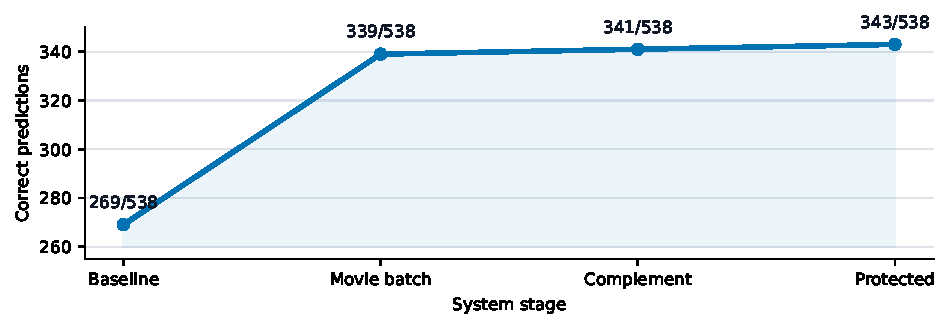
\includegraphics[width=.72\linewidth]{figures/official_progress.pdf}

  \small\textbf{Figure 1.} Historical official score chain. The large
  discontinuity coincides with a movie-batched multimodal answer source;
  later parent-preserving changes are smaller.
\end{center}

\section{Inference Pipeline}

The pipeline groups annotations, parses timestamped subtitles, samples the
chronological frame pack, sends one movie-level request, and validates the
complete JSON bank before persistence. Transient provider failures may be
retried. Missing IDs, empty answers, malformed JSON, and partial movie banks
are errors and are never silently merged.

\section{Reproducibility}

The runner accepts an OpenAI-compatible Responses endpoint and reads its key
only from a process environment variable. The conversion utility writes the
required \texttt{question\_id,prediction} CSV. The audit utility checks the
header, exact ID coverage, uniqueness, and non-empty predictions. Public and
private splits are supplied independently.

\begin{center}
\small
\begin{tabular}{ll}
\toprule
Component & Configuration \\
\midrule
Context & One movie; all questions jointly \\
Evidence & Timestamped transcript + 16 chronological JPEG frames \\
Frame encoding & Maximum side 512 px; JPEG quality 82 \\
Generation & Temperature 0; high reasoning effort \\
Output & JSON bank, then \texttt{question\_id,prediction} CSV \\
\bottomrule
\end{tabular}
\end{center}

\section{Results and Ablations}

Figure 2 reports a frozen six-movie, 60-question local diagnostic using one
semantic evaluator. Joint movie answering reaches 27/60, independent calls
18/60, and no frames 24/60. Target16 and Dense48 reach 29/60 and 30/60.
The result supports joint context; the controlled visual changes do not
establish a large standalone gain.

\begin{center}
  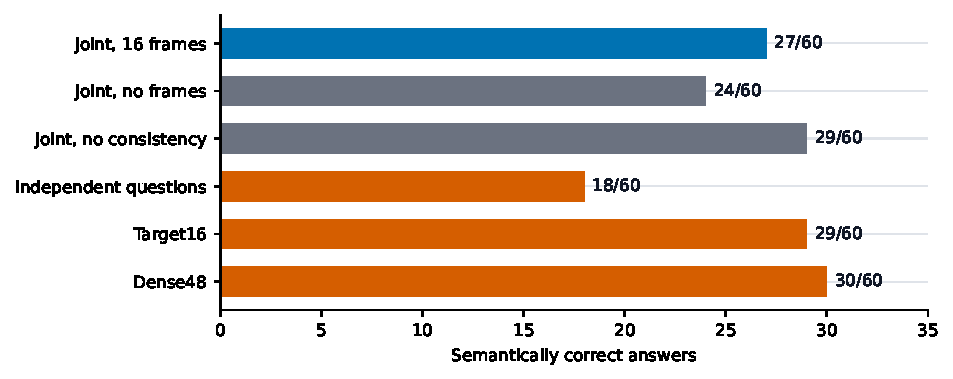
\includegraphics[width=.64\linewidth]{figures/factor_audit.pdf}

  \small\textbf{Figure 2.} Frozen factor and visual-ceiling diagnostic on six
  movies. Blue is the direct reference; gray and orange bars are controlled
  variants. These are local diagnostics, not official leaderboard scores.
\end{center}

\paragraph{Limitations.} Performance depends on transcript quality, visual
coverage, endpoint behavior, and context budget. Data and weights are external
inputs; reproduction requires authorized access and the included schema audit.
Public sources: \href{https://slomo-workshop.github.io/eccv2026/}{SLoMO},
\href{https://eval.ai/}{EvalAI}, and \href{https://huggingface.co/datasets/rghermi/sf20k}{SF20K}.

\end{document}
